\documentclass[a4paper,10pt]{report}
\renewcommand{\thesection}{}
\usepackage[utf8]{inputenc}
\usepackage{graphicx}
\usepackage{titlepic}
\usepackage{listings}
\usepackage{color}

\renewcommand\lstlistingname{Quelltext} % Change language of section name

\usepackage{tikz}
\usetikzlibrary{shapes,arrows}

%\tikzstyle{decision} = [diamond, draw, fill=white!20, 
   % text width=4.5em, text badly centered, node distance=3cm, inner sep=0pt]
%\tikzstyle{block} = [rectangle, draw, fill=white!20, 
  %  text width=5em, text centered, rounded corners, minimum height=4em]
%\tikzstyle{line} = [draw, -latex']
%\tikzstyle{cloud} = [draw, ellipse,fill=white!20, node distance=3cm,
   % minimum height=2em]
    

% Title Page

\setlength{\topmargin}{-1cm}

\title{\bf{TELECOMM. SOFTWARE LAB ELP718 \\ ASSIGNMENT NO- 6}}
\author{ANKITA GUPTA \\ ENTRY NO.- 2017JTM2021 \\ SEMESTER-I}
\titlepic{
\includegraphics[width = 50mm]{iit.png} \\ \vspace{20mm} \large{BHARTI SCHOOL OF \\
TELECOMMUNICATION TECHNOLOGY AND MANAGEMENT\\
IIT DELHI\\
INDIA}}

\lstset{ % General setup for the package
	language=Perl,
	basicstyle=\small\sffamily,
	numbers=left,
 	numberstyle=\tiny,
	frame=tb,
	tabsize=4,
	columns=fixed,
	showstringspaces=false,
	showtabs=false,
	keepspaces,
	commentstyle=\color{red},
	keywordstyle=\color{blue}
}


\begin{document}


\maketitle

\setlength{\topmargin}{-3cm}

\tableofcontents

\newpage

\section{Problem Statement 1}
 
\bf{Parity Check}
The simplest way of error detection is to append a single bit , called a parity check, to a string of data bits. 
This parity check bit has the value 1 if number of 1’s in the bit string is even and has the value 0 otherwise, i.e., Odd Parity Check.

\bf{Bit Oriented Framing}
Data Link Layer needs to pack bits into frames, so that each frame is distinguishable from another. Frames can be fixed or variable size. 
In variable size framing, we define end of frame using bit oriented approach. It uses a special string of bits, called a flag for both idle 
fill and to indicate the beginning and the ending of frames.
The string 0101 is used as the bit string or flag to indicate the end of the frame. The bit stuffing rule is to insert a 0 after each appearance
of 010 in the original data. In addition, if the frame ends in 01, a 0 would be stuffed after the 1st 0 in the actual terminating string 0101.



\subsection{Algorithm and Implementation}



\begin{itemize}

 \item Input the binary data from the user.
 \item check for the number of one's present in the data.
 \item If number of one's in data are even then append 1 at the end.
 \item Otherwise append zero at the end.
 \item Check this parity added data for bit stuffing.
 \begin{itemize}
 \item If there is presence of 010 in the parity added data then stuff a '0' after 010.
 \item Otherwise let the data as it is.
 \end{itemize}
 \item If the parity added data ends with 01 then stuff '0' in that data otherwiswe let the data as it is.
 \item add the flag at the end of the bit stuffed data to transmit.
 \item print the modified data on the terminal.
\end{itemize}



  \subsection{Input and output format}
\bf{\large{Input format}}\\

Enter binary bit data which has to be transmitted.

\bf{\large{Outpu format}}\\

Print binary bit data with parity bit.
Print the modified string received at the other end.

\newpage

\subsection{Test Cases}
\bf{sample input}\\
01010\\

\bf{sample output}\\
010101\\
010100100101\\

\bf{sample input}\\
010110\\

\bf{sample output}\\
01001100\\
010011000101\\



\subsection{Screenshots}
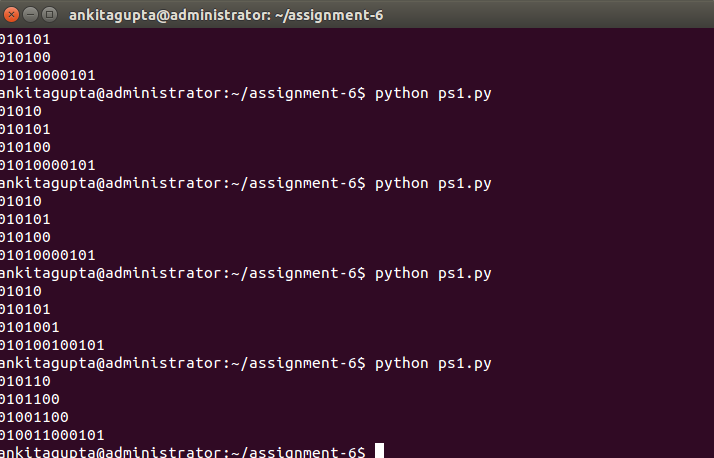
\includegraphics[width=100mm]{Screenshot from 2017-09-12 16:14:37.png}
\newpage

\section{Problem Statement 2}

3X3 Numeric Tic-Tac-Toe (Use numbers 1 to 9 instead of X’s and O’s)
One player plays with the odd numbers (1, 3, 5, 7, 9) and other player plays with the even numbers (2,4,6,8). 
All numbers can be used only once. The player who puts down 15 points in a line wins (sum of 3 numbers).
Always Player with odd numbers start the game. Once a line contains two numbers whose sum is 15 or greater, 
there is no way to complete that line, although filling in the remaining cell might be necessary to complete a different line.
Note – Line can be horizontal, vertical or diagonal

\subsection{Assumptions}
\begin{itemize}
 \item 1<=Position<=9
 \item 1<=Number<=9
 \item 1<=Sum<=15
\end{itemize}




\newpage
\subsection{Algorithm and Implementation}

\begin{itemize}
 \item To design a tic tac toe game which is played between two players.
 \item The first player can choose only odd numbers from 1-9.
 \item Second player can only choose even numbers from 1-9.
 \item The player who will attain 15 or more points will be a winner and that game should be terminated there.
 \item count should be check vertical, horizontal and diagonal.
 \item Again ask if they want to continue game or not.
\end{itemize}


\subsection{Input and output format}

\bf{input Format}
\begin{itemize}

\item Print ‘Welcome to the Game!’.    
\item Print whether it is Player 1’s or Player 2’s chance.
\item Get the position and number to be entered from user.
\item Show tic tac toe with data.
\item Continue till the game gets draw or some player wins and show result.
\item Ask user whether to continue for next game or exit.
\end{itemize}

\bf{output Format}

Welcome to the Game!\\
Player 1’s chance\\
Enter the position and number to be entered: 5,3\\
Player 2’s chance\\
Enter the position and number to be entered: 7,4\\






\subsection{Test Cases}
\subsection{Screenshots}

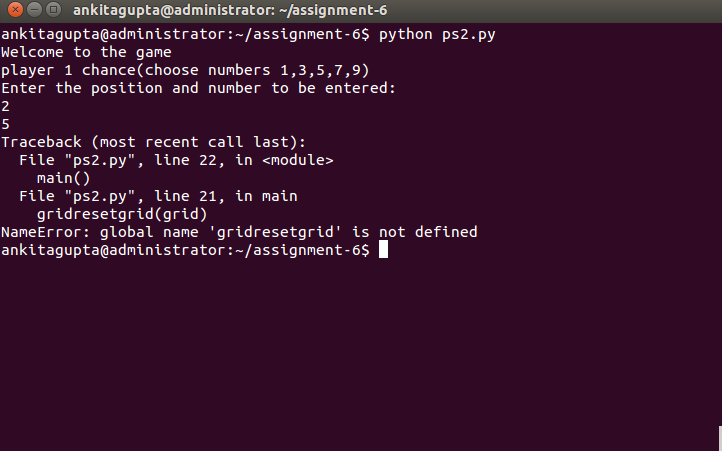
\includegraphics[width=100mm]{Screenshot from 2017-09-12 16:46:59.png}

\newpage
\section{References}
\begin{itemize}
\item https://www.tutorialspoint.com/python
\item http://www.sanfoundry.com/python-problems-solutions/
\end{itemize}

\newpage
\section{Annexure}
\bf{problem statement 1}\\
\lstinputlisting{ps1.py}
\newpage
\bf{problem statement 2}\\
\lstinputlisting{ps2.py}





\end{document}

